\section{Evaluating Visual Object Tracking}
\label{sec:EvaluatingVisualObjectTracking}

In our work, we tackle problems of \Gls{vot}, concretely \gls{mot}, for which there are no established solutions and the research is still ongoing. When it comes to evaluating \gls{mot} performance, even after many years, there is still no consensus how to approach the evaluation and subsequent comparison of multi-object trackers~\cite{Bernardin2008}.

There is one established metric, called \gls{clear} \gls{mot} metric~\cite{Bernardin2008} (further referred to as just \gls{clear}), that we will employ to evaluate the performance of a \gls{mot} system. The reasons are the following:
\begin{itemize}
    \item This metric is still considered a reasonably effective and intuitive metric to use, despite multiple proposals for improvements~\cite{CVIU_UA-DETRAC}.
    \item Numerous works in object tracking, especially people tracking, report statistics from the \gls{mot} challenges that historically have utilized this metric.
    \item From the engineering perspective, there are standard frameworks (e.g.,~\cite{pymotmetrics}) that provide evaluation of a custom \gls{mot} tracker inference with a plethora of configurations and additional metrics to evaluation. We were particularly interested in additional metrics such as the number of object switches (explained later) etc.
\end{itemize}

Bernardin et al.~\cite{Bernardin2008}, the authors of \gls{clear} discussed above, designed two crucial criteria performance metrics should meet. Here we present their list, where the first two items are considered primary, whereas the remaining are expected properties of useful metrics. Therefore, such metrics should:
\begin{enumerate}
    \item allow to assess the tracker's precision regarding how well it is capable of determining the exact object location,
    \item reflect the tracker's ability to track objects consistently, i.e., to correctly trace object trajectories such that one and only one trajectory is established per object,
    \item have as few free parameters as possible,
    \item be clear and easy to interpret while emphasizing intuitive human understanding of the tracking process,
    \item be general enough so that comparison of different types of trackers, e.g. $2$D or $3$D, is possible,
    \item contain expressive values rich in information yet not abundant in quantity.
\end{enumerate}

Considering this, they proposed a systematic approach to evaluating tracker's characteristics. For clarity, we will adopt the notation and nomenclature introduced in~\cite{Bernardin2008}.

Let $t$ denote a time for a specific frame. For each frame $t$, the multi-object tracker produces a set of hypotheses $\cbrackets{h_1, h_2, \dots, h_m}$ for a set of visible objects $\cbrackets{o_1, o_2, \dots, o_n}$. With this in mind, the evaluation procedure can be briefly described in the following pseudocode.

For each time frame $t$:
\begin{enumerate}
    \item establish the best possible correspondence between hypotheses $h_i$ and objects $o_j$, where $i = 1, 2, \dots m$ and $j = 1, 2, \dots, n$,
    \item for each determined correspondence between object and hypothesis:
    \begin{enumerate}
        \item quantify the error in estimation of the object's position,
    \end{enumerate}
    \item perform accumulation of all errors (see Fig.~\ref{fig:CLEARHypotheses}) in the found correspondences:
    \begin{enumerate}
        \item count all false negatives (misses), i.e., objects for which there was no hypothesis,
        \item count all false positives, i.e., hypotheses for which there was no object,
        \item count mismatch errors (swaps of object IDs), i.e., situations in which the hypothesis for a given object changed compared to the previous frame.
    \end{enumerate}
\end{enumerate}


\begin{figure}[t]
    \centerline{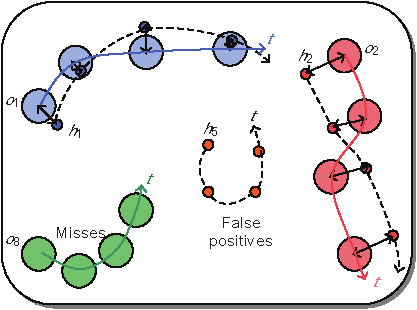
\includegraphics[width=0.6\linewidth]{figures/theoretical_foundations/clear_hypotheses_status.pdf}}
    \caption[\gls{clear} hypotheses status]{With a demonstration of a correct tracker inference at the top, the \gls{clear} \gls{mot} metric distinguishes between three fundamental types of errors, misses (false negatives), false positives and ID switches, shown in this order respectively. \externalsrc{\cite{Bernardin2008}}}
    \label{fig:CLEARHypotheses}
\end{figure}
